%%%%%%%%%%%%%%%%%%%%%%%%%%%%%%%%%%%%%%%%%%%%%%
%                insertmeeting
% 1) Title (something creative & funny?)
% 2) Date (MM/DD/YYYY)
% 3) Location (ex. Hagerty High School)
% 4) People/Committees Present 
% 5) Picture 
% 6) Start Time & Stop Time (ex. 12:30AM to 4:30PM)
%%%%%%%%%%%%%%%%%%%%%%%%%%%%%%%%%%%%%%%%%%%%%%
\insertmeeting 
	{Eye Opening CV} 
	{02/10/22} 
	{Hagerty High School}
	{James, Jensen, Samantha, Anouska, Annika, Clayton, Falon, Nathan, Ritam}
	{Images/RobotPics/robot.jpg}
	{2:30 - 4:30}
	
\hhscommittee{Software}
\noindent\hfil\rule{\textwidth}{.4pt}\hfil
\subsubsection*{Goals}
\begin{itemize}
    \item Prototype a pipeline to detect the yellow blocks during autonomous. 

\end{itemize} 

\noindent\hfil\rule{\textwidth}{.4pt}\hfil

\subsubsection*{Accomplishments}
One of our goals from the League championship was to begin increasing our autonomous score. One way to do this was scoring blocks from the warehouse onto the shipping hubs during auto. Our initial approach was to naively drive the robot into the warehouse, hoping that we would be able to intake a block before moving to place it on the shipping hub. However, after a few test runs, we realized that this system may not be as efficient as we hoped. Generallyl, the robot was able to intake a block about 50 percent of the time. We decided to brainstorm a few solutions to this problem.
One solution that we came up with was to use an OpenCV program to filter out blocks the same way we searched for the team marker at the beginning of autonomous. 
Similar to before, we began fleshing out a quick pipeline in GRIP. We started with a Gaussian blur, then an HSV threshold followed by erodes and dilates. After a quick Find Contours, the pipeline was ready to be tested with a webcam (Initial testing was done using a picture taken on a cellphone).
Upon testing with a webcam, we encountered our first issue. The plastic on the border was reflecting the yellow blocks, resulting in a double image. We managed to solve this problem by adjusting the Saturation and Value thresholds, helping to differentiate from the slightly muted colors of the reflections with the real blocks. 
After successfully detecting the blocks, we focused on calculating the heading to a block given the pixels of the rectangle. Unfortunately, we weren't able to test our pipeline with robot movement due to time constraints. So, we don't know for sure if our heading was correct. 
After much discussion and further testing, we concluded that the block pipeline may not be a big enough improvement to justify the time spent improving it. Because the blocks are thrown into the warehouse, they often appear as one big blob. This would mean we are calculating movement to the center of the blob, rather than a specific block. We could either spend more time figuring out how to automatically pick up blocks, or we could just run in and take our chances with the blocks while we try to improve other parts of the autnomous. We decided to try the second approach. 

\begin{figure}[htp]
\centering
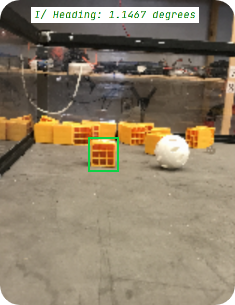
\includegraphics[width=0.95\textwidth, angle=0]{Meetings/February/02-10-22/02-10-22 1.PNG}
\caption{Our detection of a single block}
\label{fig:021022_1}
\end{figure}

\begin{figure}[htp]
\centering
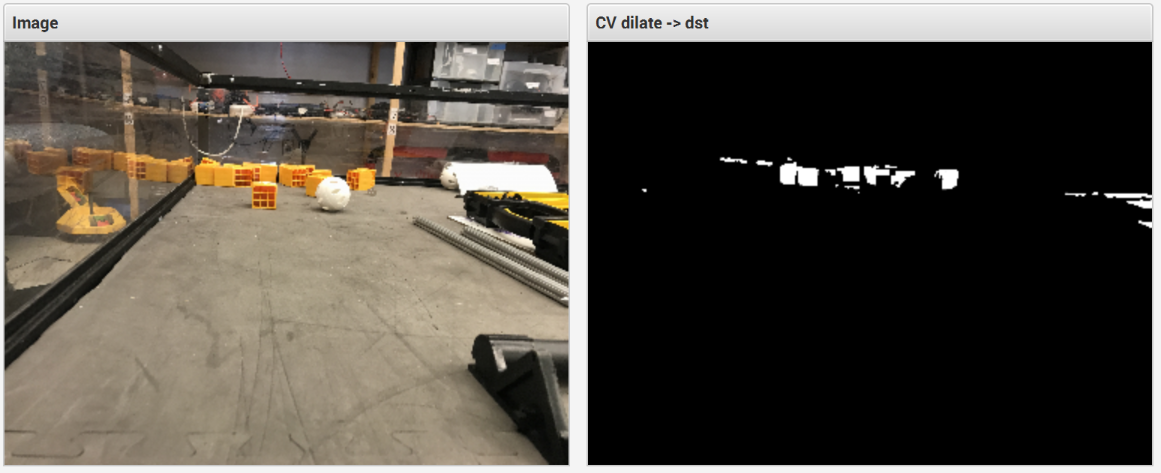
\includegraphics[width=0.95\textwidth, angle=0]{Meetings/February/02-10-22/02-10-22 2.PNG}
\caption{The large blob of blocks when tested in real life}
\label{fig:021022_2}
\end{figure}

\begin{figure}[htp]
\centering
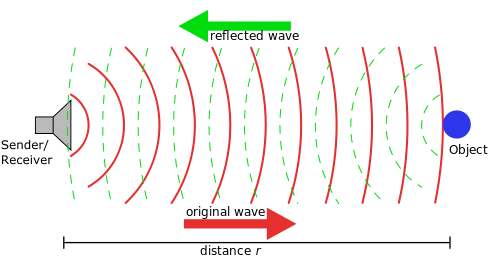
\includegraphics[width=0.95\textwidth, angle=0]{Meetings/February/02-08-22/02-08-22 3.PNG}
\caption{A diagram showing how we plan to use an ultrasonic sensor to determine the distance to the wall.}
\label{fig:021022_3}
\end{figure}


\whatsnext{
\begin{itemize}
    \item Implement ultrasonic sensor readings into the autonomous. 
\end{itemize} 
}

